\chapter{PROSPECT}

The scientific community's understanding of neutrinos has come a long way from Pauli's initial proposition of its existence in 1930. 
Though three active neutrino flavors and their behaviors are understood and well included in the Standard Model of particle physics, recent anomalies in reactor neutrino experiment results hint at the possibility of new physics. 
The discovery of an eV-scale sterile neutrino would have wide ranging impacts on the field of neutrino physics and future experiments.

The Precision Reactor Oscillation and Spectrum Experiment (PROSPECT) is designed to address the reactor antineutrino anomaly by performing a reactor-model independent search for short-baseline $\bar{\nu_{e}}$ oscillations and making a high precise measurement of the $^{235}$U $\bar{\nu_{e}}$ energy spectrum at a highly-enriched uranium (HEU) research reactor \cite{LongNIM}.
Located at the High Flux Isotope Reactor (HFIR) at Oak Ridge National Laboratory (ORNL) in Tennessee PROSPECT also demonstrates successful application of techniques for antineutrino detection at the surface with little overburden. 
PROSPECT collected data from May to December of 2018 and the first oscillation and spectrum results, with 33 and 40.3 live-days of reactor on time respectively, can be found in Ref.\cite{PhysRevLett.121.251802,Ashenfelter:2018jrx}.

\section{Experimental Site}
\subsection{HFIR}

HFIR is a compact research reactor that burns highly enriched uranium fuel ($^{235}$U), meaning that $>$ 99\% of fissions during a reactor cycle will be from $^{235}$U.
The HFIR core consists of two concentric fuel elements with an outer diameter of 0.435 m and a height of 0.508 m, surrounded by control elements and Beryllium reflectors as shown in Figure~\ref{fig:hfir}. 
The reactor typically operates at 85 MW for seven 24-day cycles per year for a duty cycle of $\sim$46\%.

\begin{figure}[t]
	\centering
	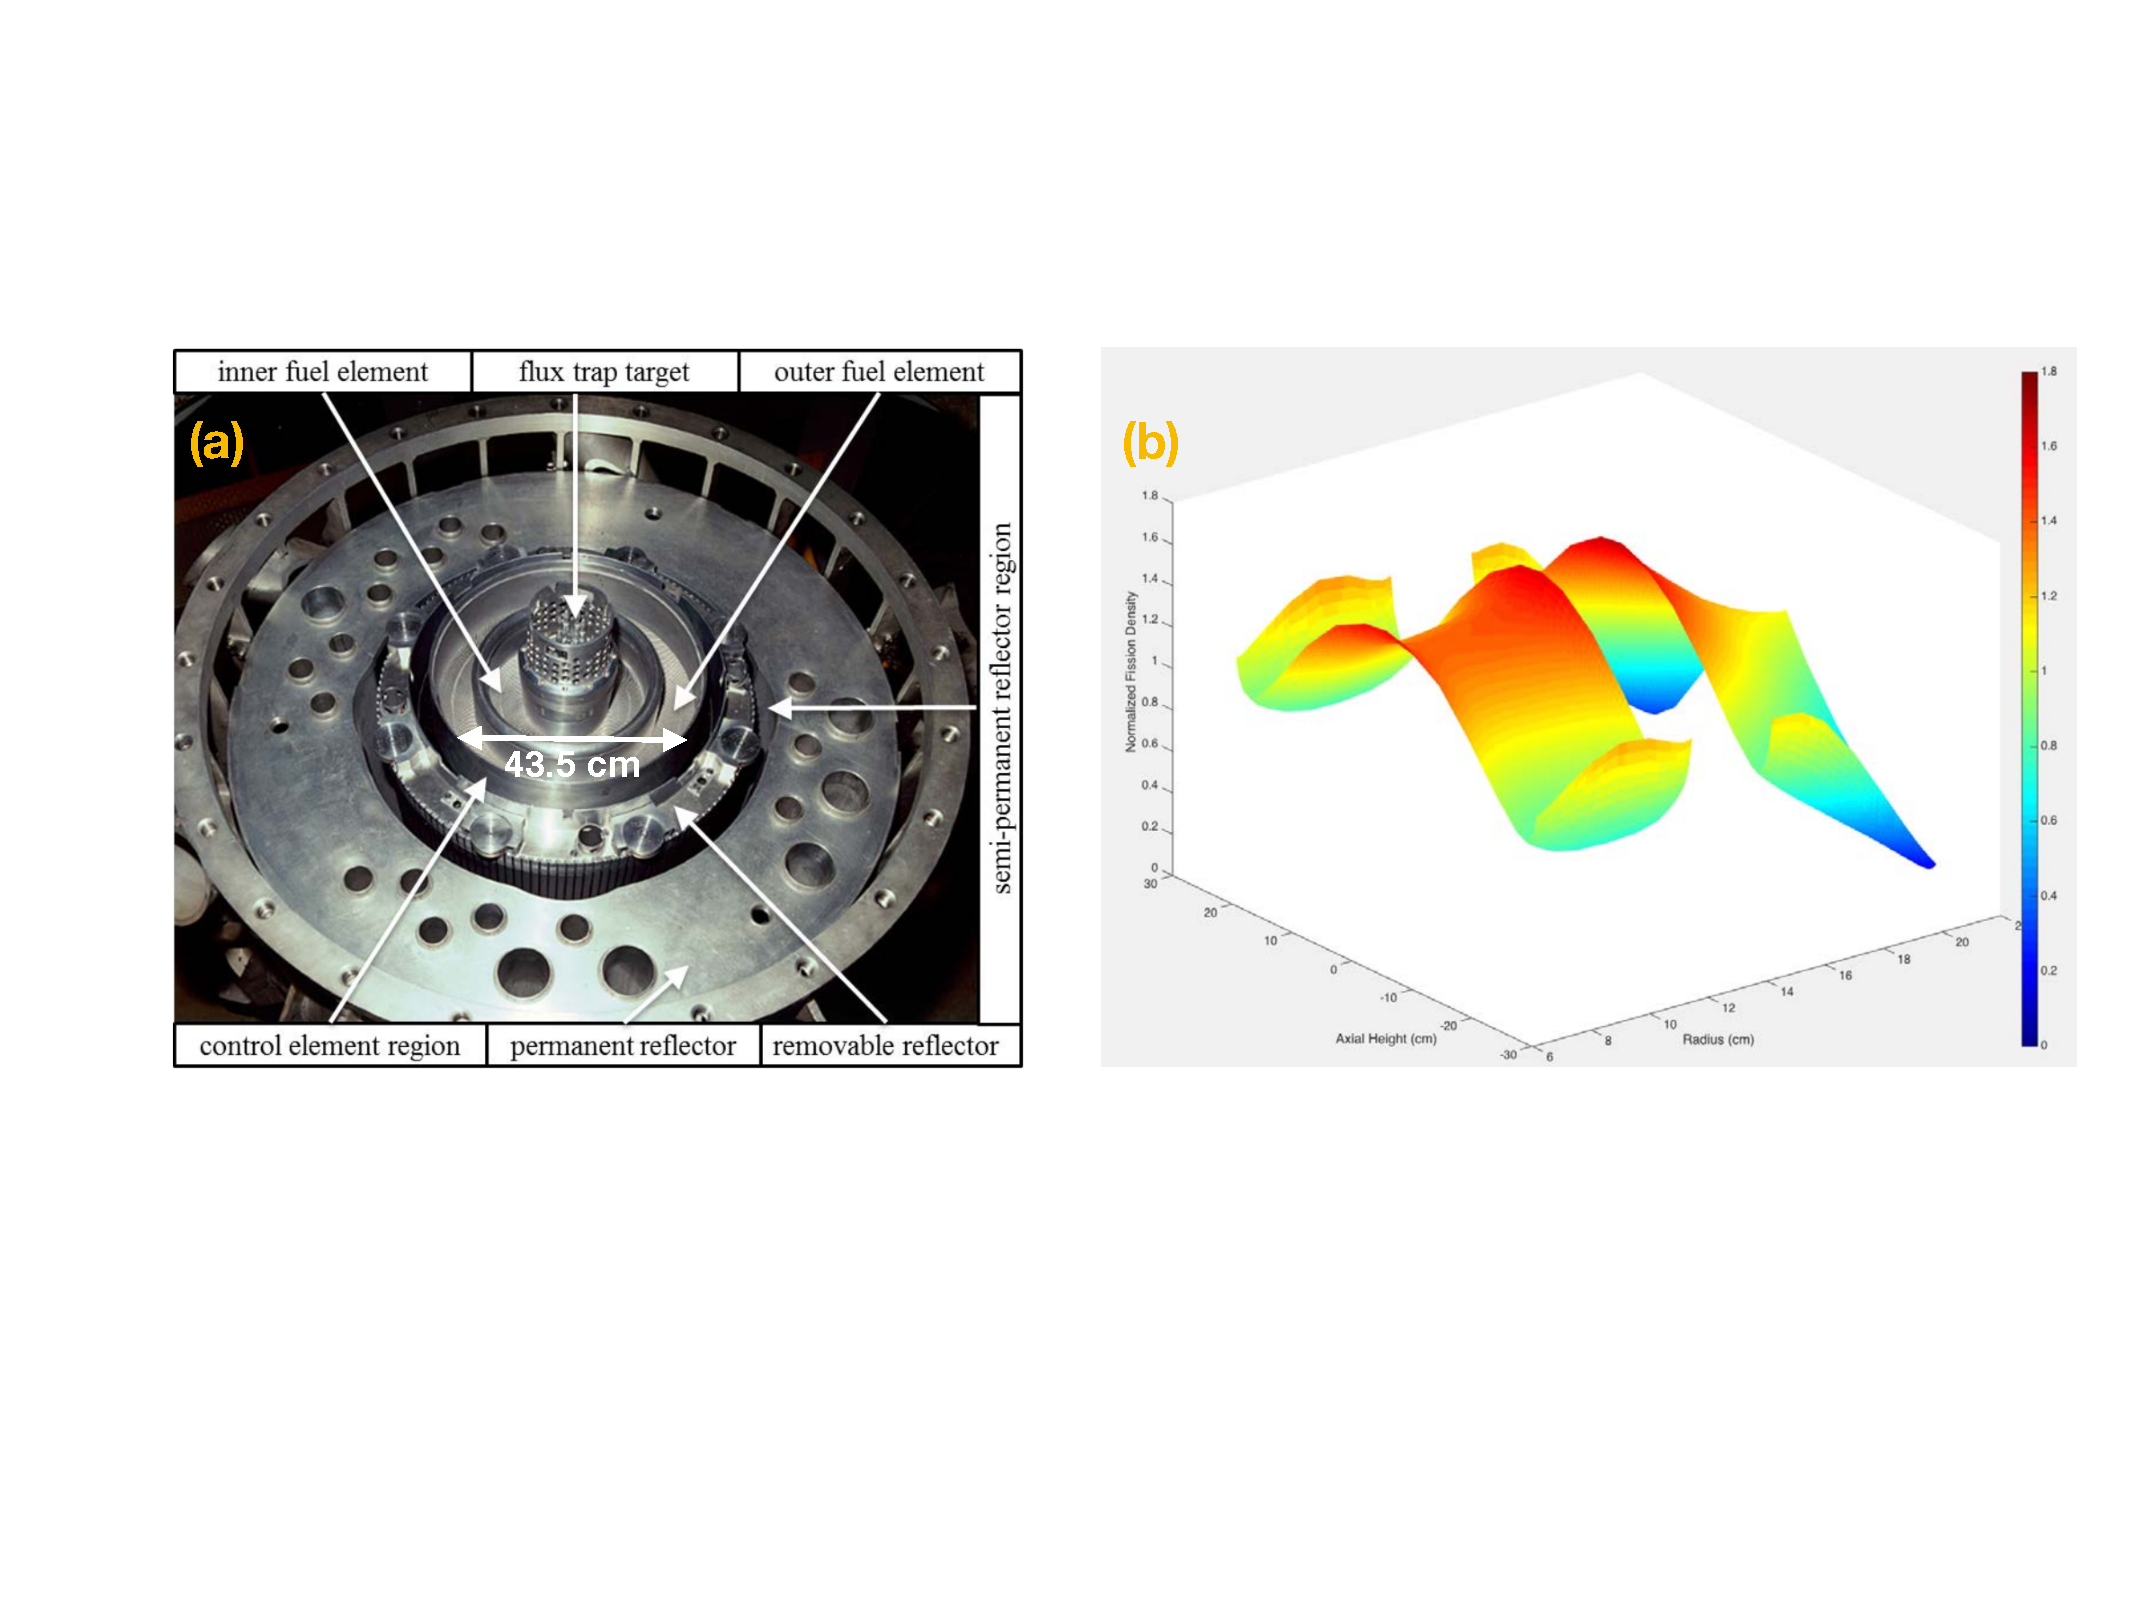
\includegraphics[width=0.9\linewidth]{tex/4-prospect-images/HFIR}
	\caption[The HFIR core and flux distribution]{(a) The HFIR core, showing the inner and outer fuel elements and the flux trap region, as well as the control elements and Beryllium reflectors. (b) The relative fission density distribution at the start of a cycle. \cite{HFIRTech}}
	\label{fig:hfir}
\end{figure}

\subsection{Backgrounds at HFIR}

The PROSPECT detector is located at ground level $\sim$7 m from the HFIR core and separated from the reactor water pool by a 1 m thick concrete wall, see Figure~\ref{fig:shielding}.
The proximity to the reactor and lack of overburden introduces a significant level of background events from the reactor and cosmogenic sources. 
These events can be classified into two categories, singles that are mainly due to gammas and coincident events from neutron recoil and captures. 
Extensive studies on the types and rate of background events at the detector site can be found in Refs.\cite{Ashenfelter:2015tpm,Heffron,Hackett}.

The largest source of gamma backgrounds was discovered to originate in the reactor pool wall, specifically an unused beam line that lies directly in front of the detector. 
In order to lower these backgrounds a lead shield wall (3.0 m wide, 2.1 m tall, and on average 0.10 m thick), along with shorter flanking walls on each side and a mini-wall placed at the opening of the beam line, was installed between the pool wall and the detector.
Other background events were shown to come from neutron beam-lines and scattering experiments existing below the detector site, but most of these are suppressed by a concrete monolith that the detector sits on.

The thermal neutron rate was measured to be $\sim$2/cm$^2$/s during reactor operation \cite{Ashenfelter:2015tpm}, so layers of shielding containing $^{10}$B, which has a large thermal neutron cross-section and minimal gamma emission, were used in the passive shielding that surrounds the detector (see Section\todo{Add section cite}). 
The locally installed shield wall, along with the addition of passive shielding, resulted in a sufficient suppression of background such that a better than one-to-one signal to background ratio was achieved. 

\begin{figure}[t]
	\centering
	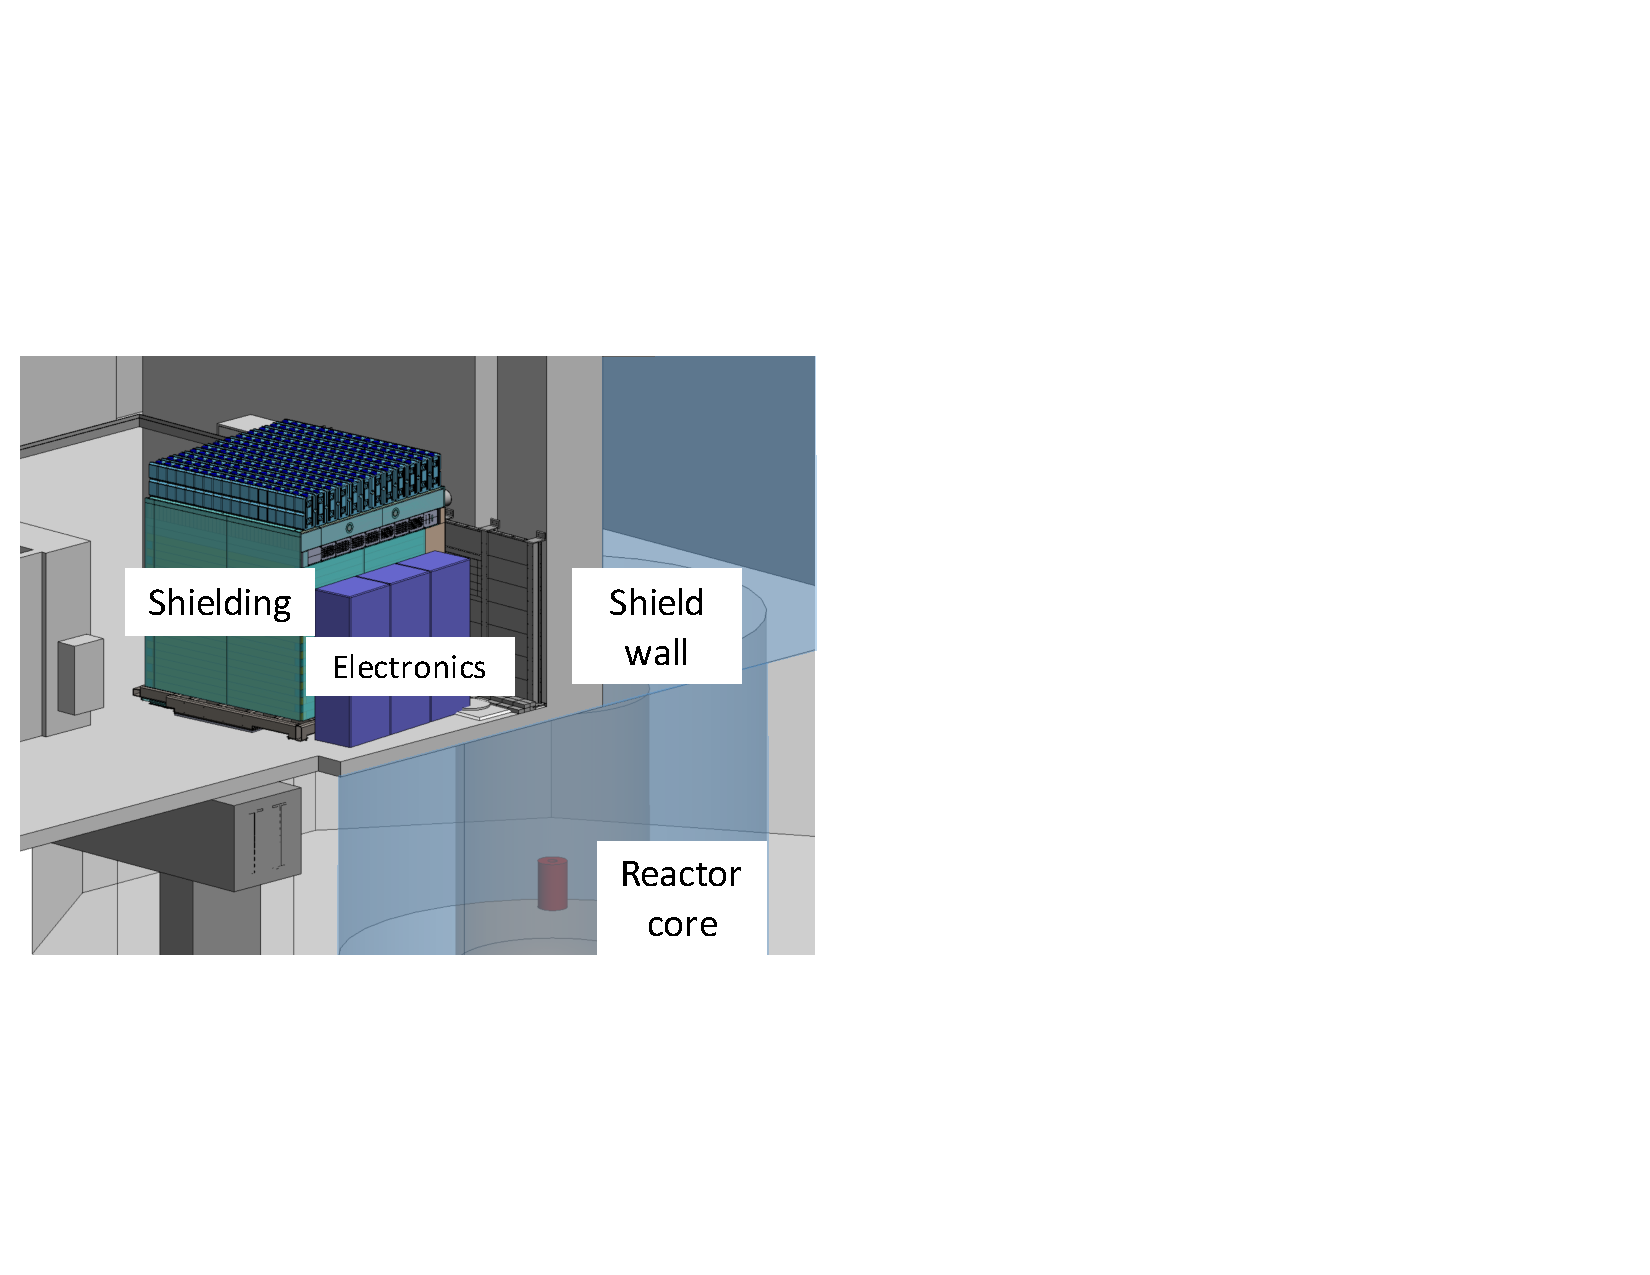
\includegraphics[width=0.5\linewidth]{tex/4-prospect-images/Shielding}
	\caption[Layout of PROSPECT at HFIR]{Layout of the PROSPECT experiment. The detector is installed in the HFIR Experiment Room next to the water pool and 5 m above the HFIR reactor core (red). The floor below contains multiple neutron beam-lines and scattering experiments.}
	\label{fig:shielding}
\end{figure}

\section{Design}

The PROSPECT antineutrino detector (AD) consists of a segmented inner detector filled with liquid scintillator (LS) viewed by photomultiplier tubes (PMT), contained in an acrylic and aluminum tanks, and surrounded by layers of passive shielding. 
The active detector is made up of a 14  $\times$ 11 array of optically separated segments, viewed on each end by a PMT enclosed in an acrylic housing and filled with LS. 
The AD is placed with the segments parallel to the reactor pool wall, $\sim$7 m from the reactor core, and measures $\sim$3 m including all shielding \todo{Check this measurement}. 
See Figure~\ref{fig:ad} for a schematic of the detector. 

\begin{figure}[t]
	\centering
	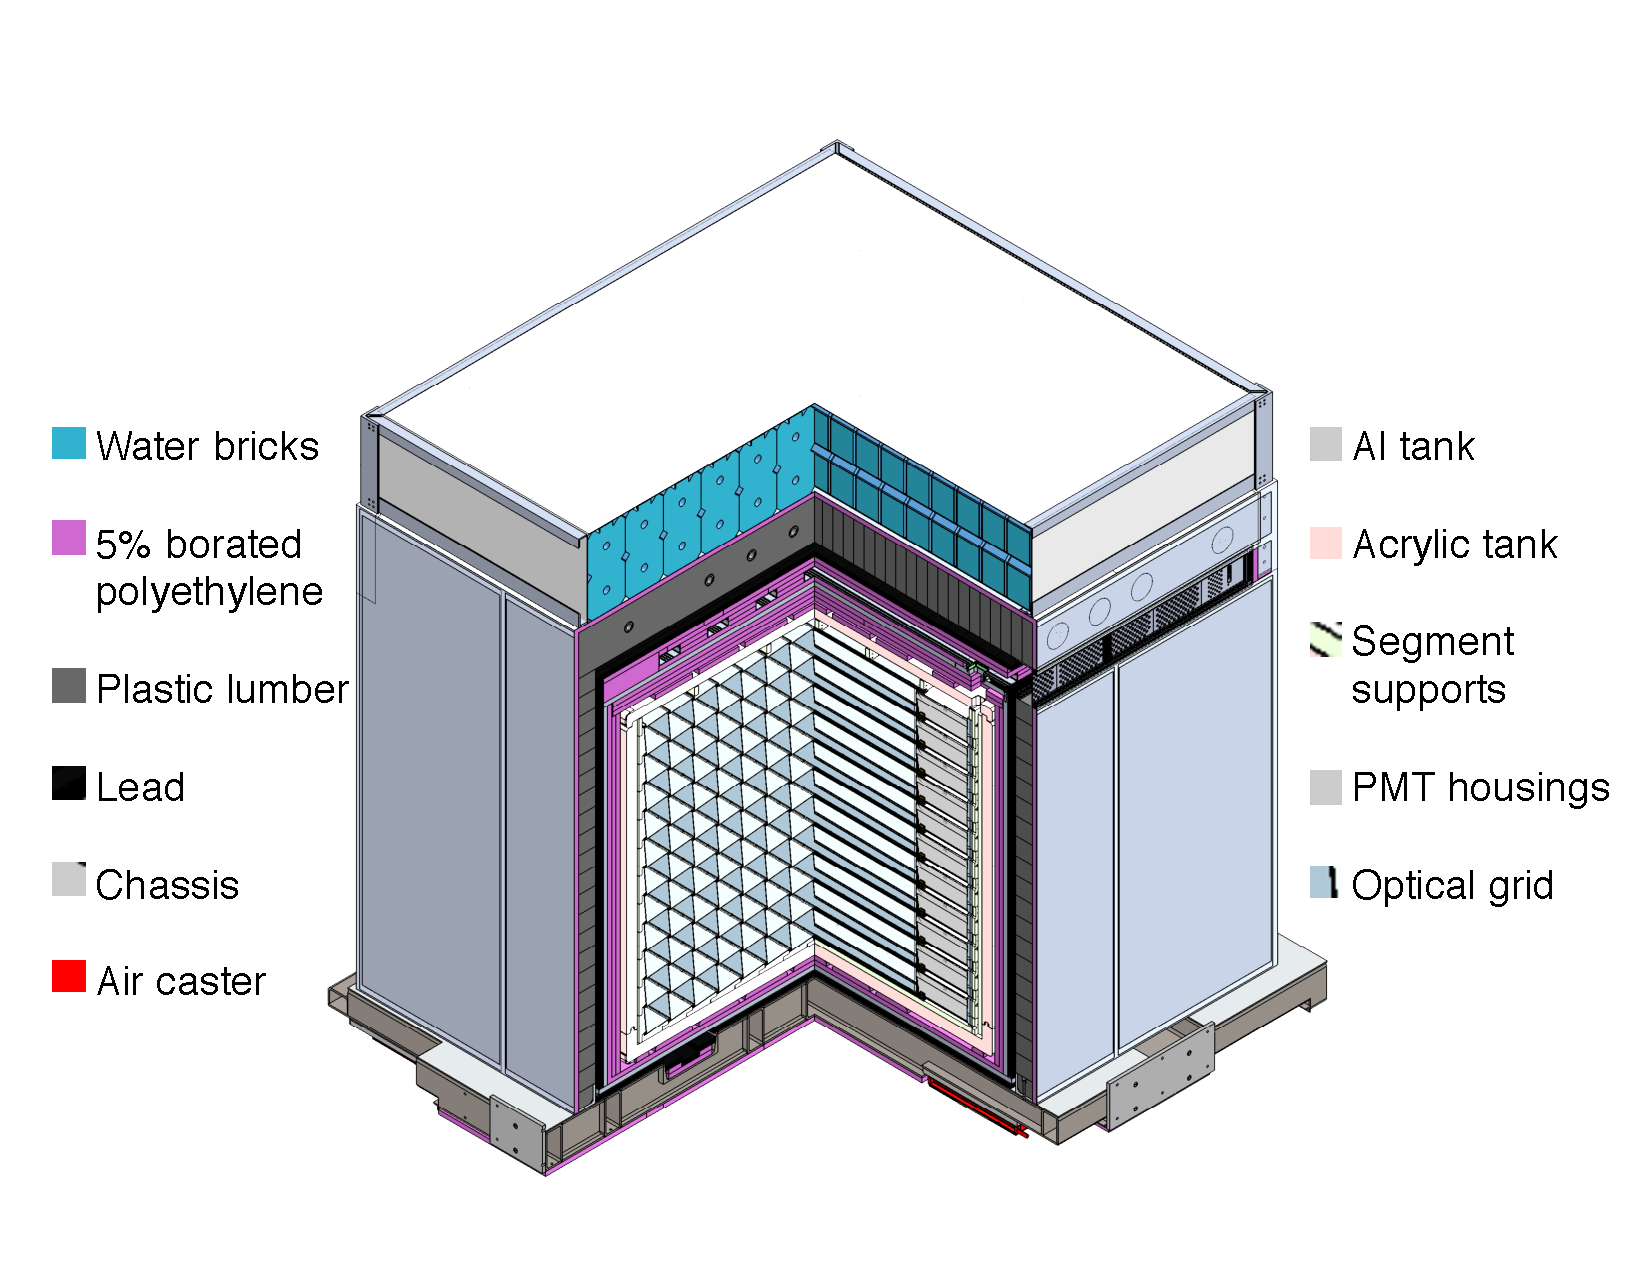
\includegraphics[width=0.8\linewidth]{tex/4-prospect-images/AD}
	\caption[Schematic of the PROSPECT detector]{A cutaway view of the PROSPECT detector, including the inner detector, outer containment vessels, and passive shielding.}
	\label{fig:ad}
\end{figure}

\subsection{Inner Detector}

\subsubsection{Optical Grid}
\subsubsection{PMT Housings}
\subsubsection{Liquid Scintillator}
\subsubsection{Segment Supports}
\subsubsection{Calibration}

\subsection{Containment Vessels and Shielding}


\section{Detecting Inverse Beta Decays}

\section{From Signal to Result}


